\documentclass{article}

\usepackage[utf8]{inputenc}
\usepackage{graphicx}
\usepackage{tikz}
\usepackage{float}
\usepackage{wrapfig,lipsum}
\usepackage{svg}
\usepackage{mathtools}
\usepackage{tabu}
\usepackage[a4paper, total={6in, 8in}]{geometry}

\begin{document}


\newcommand{\vecthreeBF}[1]{\vec{\textbf{#1}}}
\newcommand{\vecthree}[1]{\vec{#1}}

\newcommand{\parDeriv}[2]{\frac{\partial #1}{\partial #2}}
\newcommand{\parDerivS}[2]{\frac{\partial^2 #1}{\partial #2^2}}
\newcommand{\derivS}[2]{\frac{d^2 #1}{d#2^2}}

\newcommand{\dotProdBF}[2]{\vecthreeBF{#1} \cdot \vecthreeBF{#2}}
\newcommand{\dotProd}[2]{\vecthree{#1} \cdot \vecthree{#2}}

\newcommand{\crossProdBF}[2]{\vecthreeBF{#1} \times \vecthreeBF{#2}}
\newcommand{\crossProd}[2]{\vecthree{#1} \times \vecthree{#2}}


\newcommand{\fromeq}[1]{\textit{equation \ref{eq:#1}}}
\newcommand{\fromeqs}[2]{\textit{equations \ref{eq:#1} and \ref{eq:#2}}}

\newcommand{\fromfig}[1]{\textit{figure \ref{fig:#1}}}

%----../../..++++.

%%%%%%

\section{Particle Accelerators}

Particle accelerators are sophisticated scientific instruments designed to accelerate charged particles, such as electrons, protons, or ions, to high speeds and energies. 
These accelerators play a crucial role in advancing our understanding of the fundamental properties of matter and the universe. 
They are widely used in various fields of research, including particle physics, nuclear physics, materials science, and medicine.

At their core, particle accelerators utilize electromagnetic fields to impart energy to particles and control their trajectories. 
These fields are generated by intricate arrangements of magnets and RF (radiofrequency) cavities within the accelerator structure. 
By precisely controlling these fields, accelerators can propel particles to speeds close to the speed of light, enabling them to acquire high energies.

Accelerators can be categorized into two main types: linear accelerators (linacs) and circular accelerators. 
Linacs accelerate particles in a straight line, while circular accelerators use magnetic fields to bend the particle trajectory into a circular path. 

The acceleration process in accelerators involves multiple stages. Initially, particles are injected into the accelerator at a relatively low energy. 
As they progress through the accelerator, they are subjected to alternating electric fields that accelerate them, while magnetic fields guide their trajectories.
Focusing elements, such as magnetic lenses or quadrupole magnets, ensure the particles remain tightly controlled.

As particles gain energy in the accelerator, they approach relativistic speeds, where relativistic effects become significant. 
Special relativity governs the increase in mass and energy of the particles as they approach the speed of light, providing insights into the behavior of matter at high energies.

Particle accelerators are essential tools for scientific research. They enable scientists to probe the fundamental constituents of matter, study particle interactions, and explore the laws of physics. 
Accelerators have been instrumental in discovering and characterizing fundamental particles, such as quarks, leptons, and the Higgs boson. 
They also facilitate the production of high-intensity beams for applications in material science, radiotherapy, and industrial processes like particle irradiation and sterilization.

% TODO : ADD CIRCULAR AND LINEAR ACCELERATOR PICTURES HERE
\begin{figure}[H]
    \centering
    
\includegraphics[scale=0.75]{../../../figures/to_be_added.png}
    \caption{A circular accelerator}
\end{figure}

\begin{figure}[H]
    \centering
    
\includegraphics[scale=0.75]{../../../figures/to_be_added.png}
    \caption{A linear accelerator}
\end{figure}

\subsection{Key Concepts}

\begin{itemize}
    \item Phase Stability
    \item Phase Lag
    \item Shunt Impedance
    
\end{itemize}

\subsection{Acceleration Cavities}
Radiofrequency (RF) cavities, also known as accelerating cavities or resonant cavities, are key components in particle accelerators. 
These cavities generate strong electromagnetic fields at specific frequencies to accelerate charged particles through clever engineering.

RF cavities are typically hollow metallic structures made of or coated with high-conductivity materials such as copper. 
They are designed to resonate at a specific frequency, which is determined by the size and shape of the cavity. 
The cavity is often cylindrical or spherical in shape, and its inner surface is polished to minimize energy losses through resistive heating.
The RF cavity is designed to be resonant, meaning that it naturally amplifies the electric fields at its resonant frequency. 
The resonant frequency is determined by the cavity's dimensions and the speed of light in the cavity material.

To achieve efficient energy transfer to the particles, the RF cavity is driven by an external RF power source operating at the resonant frequency. 
The power source supplies radiofrequency energy to the cavity, which causes the electric fields inside the cavity to oscillate at the desired frequency. 
These oscillating fields then transfer energy to the passing particles, increasing their kinetic energy by pushing and pulling on the charged particles as they pass through the cavity. 

In addition to accelerating the particles, RF cavities are often designed to provide focusing forces. 
By carefully shaping the cavity and adjusting the electromagnetic fields, the particles can experience focusing effects as they pass through the cavity. 
This helps to maintain a tight and controlled beam. To ensure efficient acceleration, it is essential to maintain phase stability. 
This means that the particles should experience the strongest electric fields at the correct time during their passage through the cavity. 
Precise timing and synchronization of the RF power source with the particle beam are crucial to achieve phase stability and maximize energy transfer.
% TODO : ADD RF CAVITY PICTURE HERE
\begin{figure}[H]
    \centering
    
\includegraphics[scale=0.75]{../../../figures/to_be_added.png}
    \caption{A rf cavity used in KAHVELab}
\end{figure}

\subsection{Steerer Magnets}
Steerer magnets, also known as dipole magnets or bending magnets, are fundamental components used in particle accelerators to control the trajectory of charged particles. 
They utilize the Ampere's Law to exert a magnetic field that interacts with the charged particles in the accelerator. 

According to the Lorentz Force Law ( $\textit{Section \ref{sec:lorentz-force}}$ ), when a charged particle moves through a magnetic field, it experiences a force perpendicular to both its velocity 
vector and the magnetic field direction. This force causes the particle's trajectory to curve, resulting in a bending effect.

% TODO : ADD STEERER MAGNET PICTURE HERE
\begin{figure}[H]
    \centering
    
\includegraphics[scale=0.75]{../../../figures/to_be_added.png}
    \caption{A steerer magnet used in KAHVELab}
\end{figure}

\subsection{Rhodotron Accelerator}

Rhodotron Accelerator is a type of particle accelerator that was proposed by \textit{Jacques POTTIER} in his publication \textit{A new type of rf electron accelerator:The Rhodotron} in 1989 \cite{rhodo_pottier}. 
First prototype was built at CEA Saclay later in 1992 \cite{rhodo_prototype}. Its named after the greek word for rose, \textit{rhodos}, due to the shape of the design \cite{rhodos}.

The design of a rhodotron mainly consists of a coaxial cylindrical RF cavity and steerer magnets surrounding it. RF cavity is fed by an external RF source, accelerating the electrons entering from an attached electron gun.

\subsubsection{Cavity of a Rhodotron}

Coaxial design of the cavity concentrates the electric field, while the magnetic field diminishes in the middle of the cylinders. 
Therefore the electrons are injected and accelerated in the plane of zero magnetic field where the electric field is strongest.
% TODO : ADD SUPERFISH AND CST SIMULATIONS OF A SIMPLE RHODOTRON CAVITY

\begin{figure}[H]
    \centering
    
\includegraphics[scale=0.75]{../../../figures/to_be_added.png}
    \caption{SUPERFISH simulation of a coaxial cavity}
\end{figure}

\begin{figure}[H]
    \centering
    
\includegraphics[scale=0.75]{../../../figures/to_be_added.png}
    \caption{CST simulation of a coaxial cavity}
\end{figure}

With the expectation that the electrons will accelerate to speeds $>=0.9 c$ after the first pass, a rhodotron cavity is designed so that the length of the path between successive passes is an integer multiple of $\lambda$, wavelength of the RF field ($l=p\lambda \label{eq:lpl}$).
This constraint helps with  phase stability and synchronization of the beam.

In the table below, optimized characteristics of a rhodotron cavity can be observed. 
\begin{figure}[H]
    \centering
    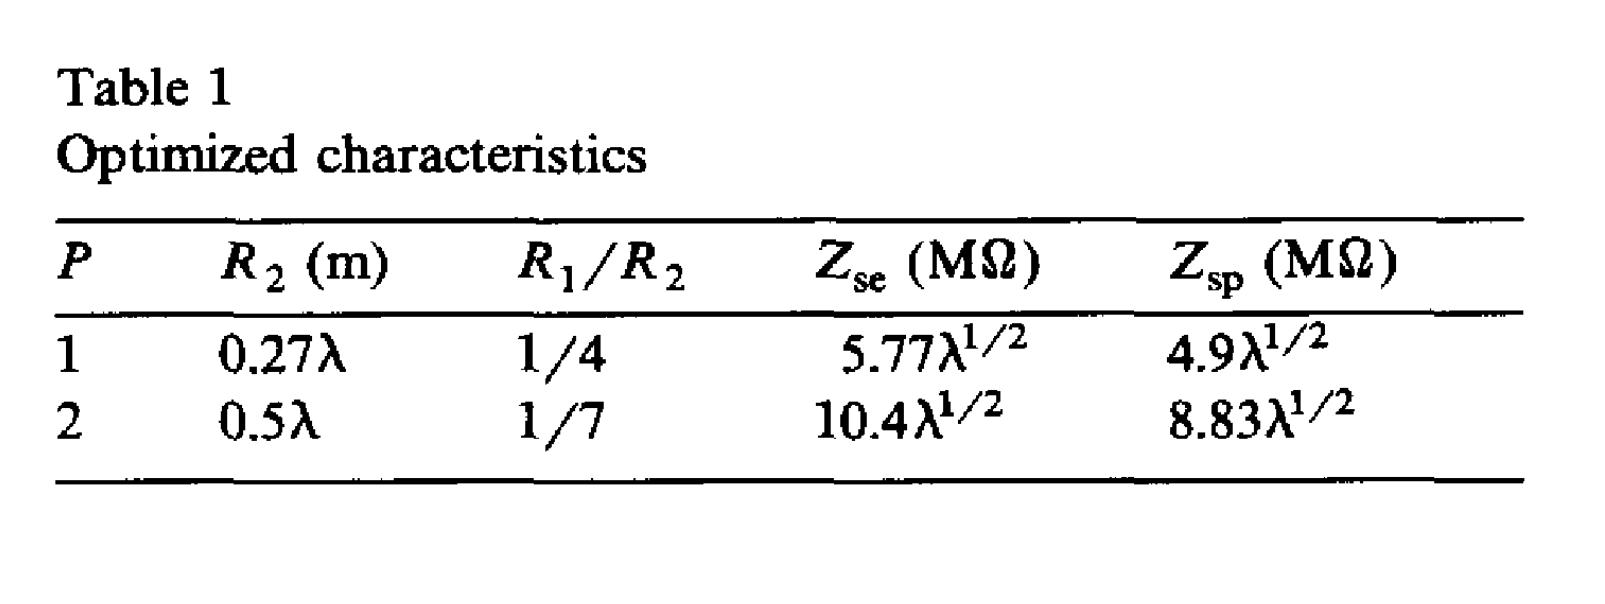
\includegraphics[width=.9\textwidth]{../../../figures/pottier_table1.png}
    \caption{Optimized characteristics of a rhodotron cavity \cite{rhodo_pottier}}
    \label{fig:pottier_table1}
\end{figure}

Here, $p$ is the integer multiplier in the equation ($l=p\lambda \label{eq:lpl}$) mentioned above, $R_1$ is the radius of the inner cylinder, $R_2$ is the radius of the outer cylinder, 
$Z_{se}$ is effective shunt empedance, $Z_{sp}$ is practical shunt empedance which was taken to be $0.85 Z_{se}$.

Energy gain after each pass can be calculated by the following formula \cite{rhodo_pottier}
\begin{equation}
    \label{eq:W_gain_each_pass_pottier}
    W_1 = Z_{sp}^{1/2} P^{1/2} cos \phi  
\end{equation}

Where $P$ is the dissipated power, $\phi$ is the phase lag, taken as $15^\circ$ \cite{rhodo_pottier}. 

Considering $Z_{sp} \propto \lambda^{1/2}$, \,\,\, $W_1 \propto \lambda^{1/4}$, \,\,\,   $V \propto \lambda^3$, where $V$ is the volume of the cavity, implementing the $p=1$ design in \fromfig{pottier_table1} is much more space efficient.
\begin{figure}[H]
    \centering
    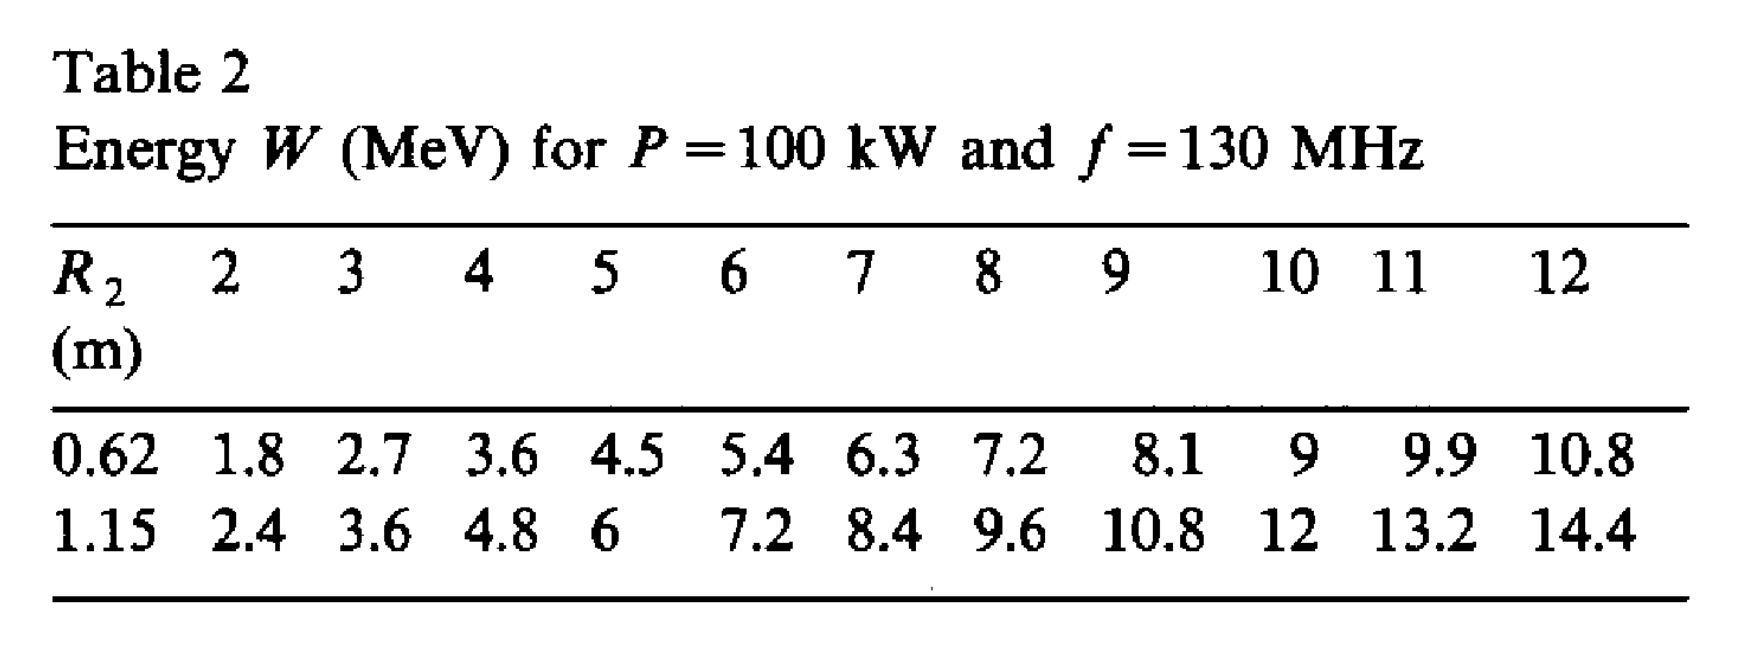
\includegraphics[width=.9\textwidth]{../../../figures/pottier_table2.png}
    \caption{Energy of a synchronous electron after each pass for both $p=1$ and $p=2$ \cite{rhodo_pottier}}
    \label{fig:pottier_table2}
\end{figure}

Total energy gain after n passes $W$ can then be found by \fromeq{W_gain_each_pass_pottier}, taking $p=1$, i.e $R_2 = 0.27 \lambda$.
\begin{equation}
    \label{eq:W_total_gain_pottier}
    W \approx 2.3 \lambda^{1/4} P^{1/2} n
\end{equation}

\subsubsection{Acceleration cycle of Rhodotron}

Electrons undergo four different stages during a single pass. 
They are accelerated between the cylinderical plates and are shielded from the changing RF field while inside the inner cylinder and outside the cavity. 

\begin{description}
    \item[First acceleration] Electrons in the rhodotron cavity are accelerated by the electric field created between two coaxial cylinders, towards the inner cylinder when they are ejected into the cavity.
    \item[Inner shielding] While inside the inner cylinder, the cylinder acts as a faraday cage and shields the electrons inside while the electric field is being reversed.
    \item[Second acceleration] Once the electrons leave the inner cylinder, they accelerate towards the outer cylinder by the reversed electric field until they leave the cavity.
    \item[Magnets] After leaving the cavity, an electromagnet placed in their path steers the electrons back into the cavity in which time the electric field changes the direction again.
\end{description}

This cycle can be repeated as long as real world constraints such as; placements and dimentions of the electromagnets, power requirements due to increasing magnetic field in order for sharper turns, can be overcomed.
After desired amount of pass has been completed, the electrons exit the accelerator.

This process is explained further in the following figures where $T$ is the period of the electric field.
% TODO : ADD ACCELERATION PROCESS OF RHODOTRON FIGURES HERE
\begin{figure}[H]
    \centering
    
\includegraphics[scale=0.75]{../../../figures/to_be_added.png}
    \caption{$[0, \frac{T}{4}]$ time frame of a rhodotron}
\end{figure}

\begin{figure}[H]
    \centering
    
\includegraphics[scale=0.75]{../../../figures/to_be_added.png}
    \caption{$[\frac{T}{4}, \frac{T}{2}]$ time frame of a rhodotron}
\end{figure}

\begin{figure}[H]
    \centering
    
\includegraphics[scale=0.75]{../../../figures/to_be_added.png}
    \caption{$[\frac{T}{2}, \frac{3T}{4}]$ time frame of a rhodotron}
\end{figure}

\begin{figure}[H]
    \centering
    
\includegraphics[scale=0.75]{../../../figures/to_be_added.png}
    \caption{$[\frac{3T}{4}, T]$ time frame of a rhodotron}
\end{figure}



%%%%%%

\begin{thebibliography}{9}
    \bibitem{rhodo_pottier}
    Jacques Pottier,
    \emph{A new type of rf electron accelerator: The rhodotron},
    Nuclear Instruments and Methods in Physics Research Section B: Beam Interactions with Materials and Atoms,
    Volumes 40–41, Part 2,
    1989,
    Pages 943-945,


    \bibitem{rhodo_prototype}
    J.M. Bassaler, J.M. Capdevila, O. Gal, F. Lainé, A. Nguyen, J.P. Nicolaï, K. Umiastowski,
    \emph{Rhodotron: an accelerator for industrial irradiation},
    Nuclear Instruments and Methods in Physics Research Section B: Beam Interactions with Materials and Atoms,
    Volume 68, Issues 1–4,
    1992,
    Pages 92-95,A:

    \bibitem{rhodos}
    Y. Jongen. (2001). \emph{Manufacturing of Electron Accelerators}. Ion Beam Applications s.a. (IBA) Chemin du Cyclotron 3, B-1348 Louvain-la-Neuve, Belgium.
\end{thebibliography}

\end{document}